% -*- coding: utf-8 -*-

% Ausgabe des Literaturverzeichnisses; ohne weitere Optionen werden nur die
% Bücher und Artikel ausgegeben, die in der Arbeit auch zitiert werden.
\printbibliography

% markiert den Anfang des Anhangs
\appendix

% ein Kapitel, das nicht numeriert, aber trotzdem ins Inhaltsverzeichnis
% aufgenommen wird
\clearpage
\section*{Anhang}
\begin{figure}[p]
	\centering
	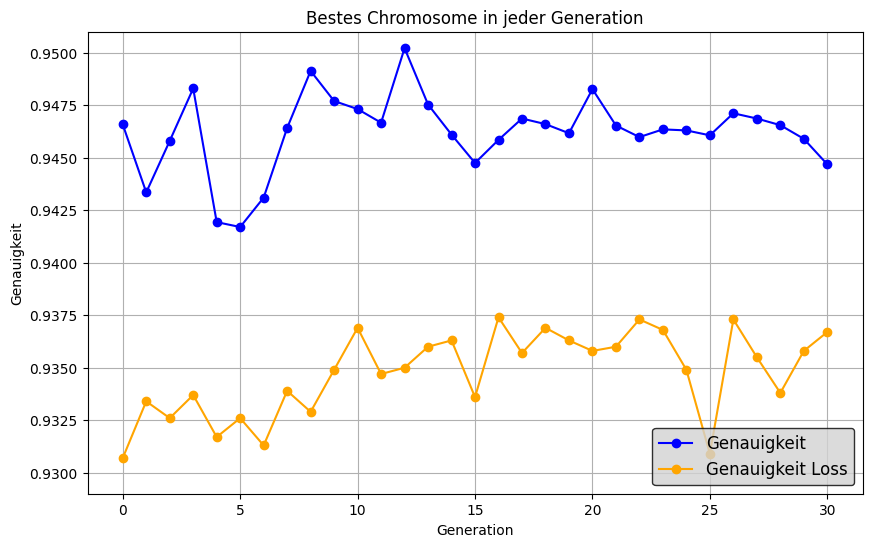
\includegraphics[width=1\linewidth]{acc.png}
	\caption{Lauf mit Priorisierung der Exploitation: Höchste Genauigkeit pro Generation}
	\label{fig:enter-label}
\end{figure}

\begin{figure}[p]
	\centering
	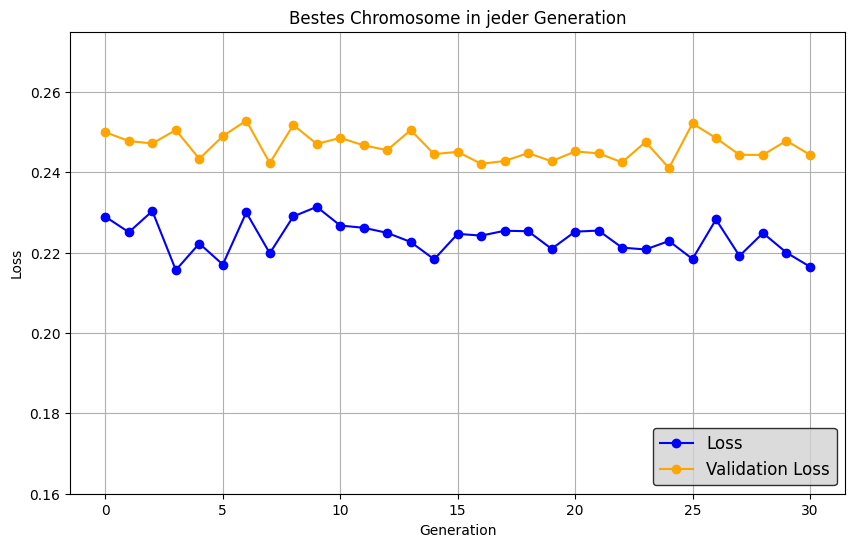
\includegraphics[width=1\linewidth]{loss_explore.png}
	\caption{Lauf mit Priorisierung der Exploration: Geringster Fehler pro Generation}
	\label{fig:enter-label}
\end{figure}

\begin{figure}[p]
	\centering
	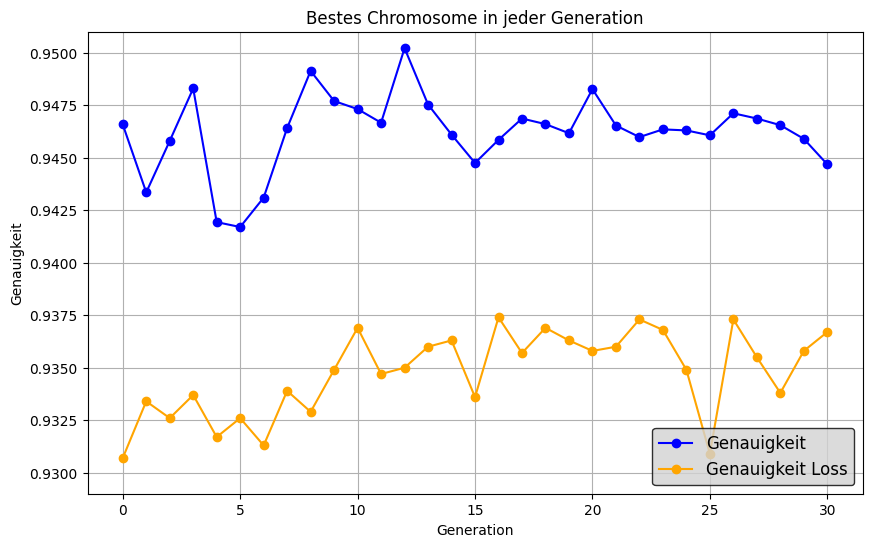
\includegraphics[width=1\linewidth]{acc.png}
	\caption{Lauf mit Priorisierung der Exploration: Höchste Genauigkeit pro Generation}
	\label{fig:enter-label}
\end{figure}


Der Sourcecode steht auf Github zur Verfügung:\\
\url{https://github.com/jonasmetzger2000/KI-STG-GI-Neural-Network-Optimizer}

% neue Seite
\clearpage

% keine Seitenzahl
\thispagestyle{empty}

% keine Nummerierung, keine Aufnahme ins Inhaltsverzeichnis
\section*{Eigenständigkeitserklärung}

% Hier müssen Sie natürlich den Titel der Arbeit sowie Ort und Datum ersetzen:
Hiermit versichere ich, dass ich die vorliegende Bachelorarbeit mit dem Titel
\begin{center}
  \textbf{Optimierung der Hyperparameter eines Neuronalen Netzes durch einen evolutionären Algorithmus}
\end{center}
selbstständig und nur mit den angegebenen Hilfsmitteln verfasst habe.  Alle
Passagen, die ich wörtlich aus der Literatur oder aus anderen Quellen wie
z.\,B. Internetseiten übernommen habe, habe ich deutlich als Zitat mit Angabe
der Quelle kenntlich gemacht.

\vspace{2cm}

Hamburg, 2. August 2024
